\subsection{Evaluation Methodology:}
To evaluate the application there will be two methods used both based upon methods found in the literature review.
The first is a visual test at time steps during the running of the program.
This will hopefully showcase the formation and deformation of clouds and the generation of rain.
Figure 3.1 shows \citet{DobashiEtAl00} results in the manner describe here.
In the appendix Figure 6.2 to Figure 6.4 show the results from other models.
This method has been chosen because it shows of the purpose of the project which is to have visually realistic clouds simulated at real time with the creation of rain. \\
\begin{figure}[h!]\label{fig:Simple Realistic Animation of Clouds}
  \centering
  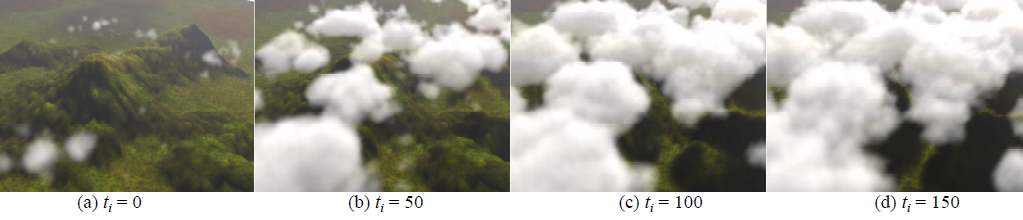
\includegraphics[width=140mm]{images/Simple_Realistic_Animation_of_Clouds.PNG}
  \caption{\citet{DobashiEtAl00}}
\end{figure}

The other method that will be used is to test how much resources are being used by the application.
\citet*{MHarris01}, and \citet{Elek12} both used this method when evaluating their models.
This form of evaluation will be used to test how efficient the application is when running in real time as well as concerns like the size of grid that can be used.
This can be accomplished using NSight Visual Studio Edition for debugging CUDA and profiling the application.